\documentclass{beamer}
\usetheme{CambridgeUS}
\usecolortheme{dolphin}
\usepackage{tikz}
\usepackage{amsmath}
\usepackage{media9}

\title{Introdução a Processos Estocásticos}
\subtitle{Exemplo: Processo de Poisson}
\author{Prof. Jair Donadelli}
\institute{UFABC}
\date{\today}

\begin{document}

%------------------------------------------------
\begin{frame}
  \titlepage
\end{frame}
%------------------------------------------------

\begin{frame}{Intuição: Chegada de Clientes}
Imagine um café: os clientes chegam em instantes aleatórios.
\pause
\begin{itemize}
  \item O número de chegadas até o tempo $t$ é uma variável aleatória $X(t)$.
  \pause
  \item Cada dia observamos uma trajetória diferente do processo.
\end{itemize}

\pause
\begin{center}
\begin{tikzpicture}[scale=0.9]
  % eixo do tempo
  \draw[->] (0,0) -- (10,0) node[right] {$t$};
  % marcas de chegadas
  \foreach \x in {1.5,3,4.8,6.2,8.5}{
    \draw[red,thick] (\x,0) -- (\x,0.4);
    \node[red,above] at (\x,0.4) {X};
  }
\end{tikzpicture}
\end{center}
\end{frame}
%------------------------------------------------

\begin{frame}{Trajetória do Processo de Poisson}
\begin{itemize}
  \item O processo é \textbf{contínuo no tempo}.
  \pause
  \item Mas o espaço de estados é \textbf{discreto}.
  \pause
  \item Cada chegada aumenta $X(t)$ em +1.
\end{itemize}

\pause
\begin{center}
\begin{tikzpicture}[scale=0.9]
  % eixo
  \draw[->] (0,0) -- (10,0) node[right] {$t$};
  \draw[->] (0,0) -- (0,5) node[above] {$X(t)$};

  % escada
  \only<4->{\draw[thick,blue] (0,0) -- (1.5,0);}
  \only<5->{\draw[thick,blue] (1.5,1) -- (3,1);}
  \only<6->{\draw[thick,blue] (3,2) -- (4.8,2);}
  \only<7->{\draw[thick,blue] (4.8,3) -- (6.2,3);}
  \only<8->{\draw[thick,blue] (6.2,4) -- (8.5,4);}
  \only<9->{\draw[thick,blue] (8.5,5) -- (10,5);}

  % pontos de salto
  \only<5->{\fill[blue] (1.5,1) circle (2pt);}
  \only<6->{\fill[blue] (3,2) circle (2pt);}
  \only<7->{\fill[blue] (4.8,3) circle (2pt);}
  \only<8->{\fill[blue] (6.2,4) circle (2pt);}
  \only<9->{\fill[blue] (8.5,5) circle (2pt);}
\end{tikzpicture}
\end{center}
\end{frame}
%------------------------------------------------

\begin{frame}{Distribuição de $X(t)$}
\uncover<1->{Para um processo de Poisson com taxa $\lambda > 0$:}
\[
\uncover<2->{X(t) \sim \text{Poisson}(\lambda t)}
\]
\uncover<3->{Isto significa que}
\[
\uncover<3->{\mathbb{P}[X(t) = k] = e^{-\lambda t} \frac{(\lambda t)^k}{k!}, 
\quad k = 0,1,2,\dots}
\]

\pause
\begin{center}
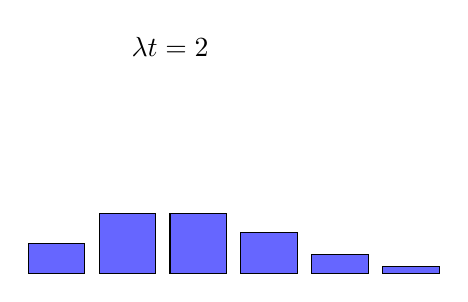
\begin{tikzpicture}[scale=0.9]
  \foreach \k/\v in {0/0.14,1/0.28,2/0.28,3/0.19,4/0.09,5/0.03}{
    \uncover<4->{\draw[fill=blue!60] (\k,0) rectangle (\k+0.8,\v*3);}
  }
  \node at (2,3.2) {$\lambda t = 2$};
\end{tikzpicture}
\end{center}
\end{frame}
%------------------------------------------------

\begin{frame}{Conceitos-Chave do Processo de Poisson}
\begin{itemize}
  \item<1-> \textbf{Processo estocástico}: coleção $\{X(t), t \geq 0\}$.
  \item<2-> \textbf{Tempo contínuo, estados discretos}.
  \item<3-> \textbf{Trajetórias}: funções escada, não-decrescentes.
  \item<4-> \textbf{Propriedades}:
    \begin{itemize}
      \item<5-> Incrementos independentes.
      \item<6-> Incrementos estacionários.
    \end{itemize}
\end{itemize}
\end{frame}
%------------------------------------------------

\begin{frame}{Animação: Processo de Poisson}
Clique para rodar a animação da trajetória:

\includemedia[
  activate=onclick,
  width=0.8\linewidth,
  height=0.6\linewidth,
  addresource=poisson_trajetoria.mp4,
  flashvars={source=poisson_trajetoria.mp4}
]{}{VPlayer.swf}
\end{frame}
\end{document}
